\begin{landscape}
\subsection{\centering Oral Argument -- Time for Arguments}

\begin{figure}[H]
\centering
\caption{Total Time Speaking (Minutes) by Justice (OT2023)}
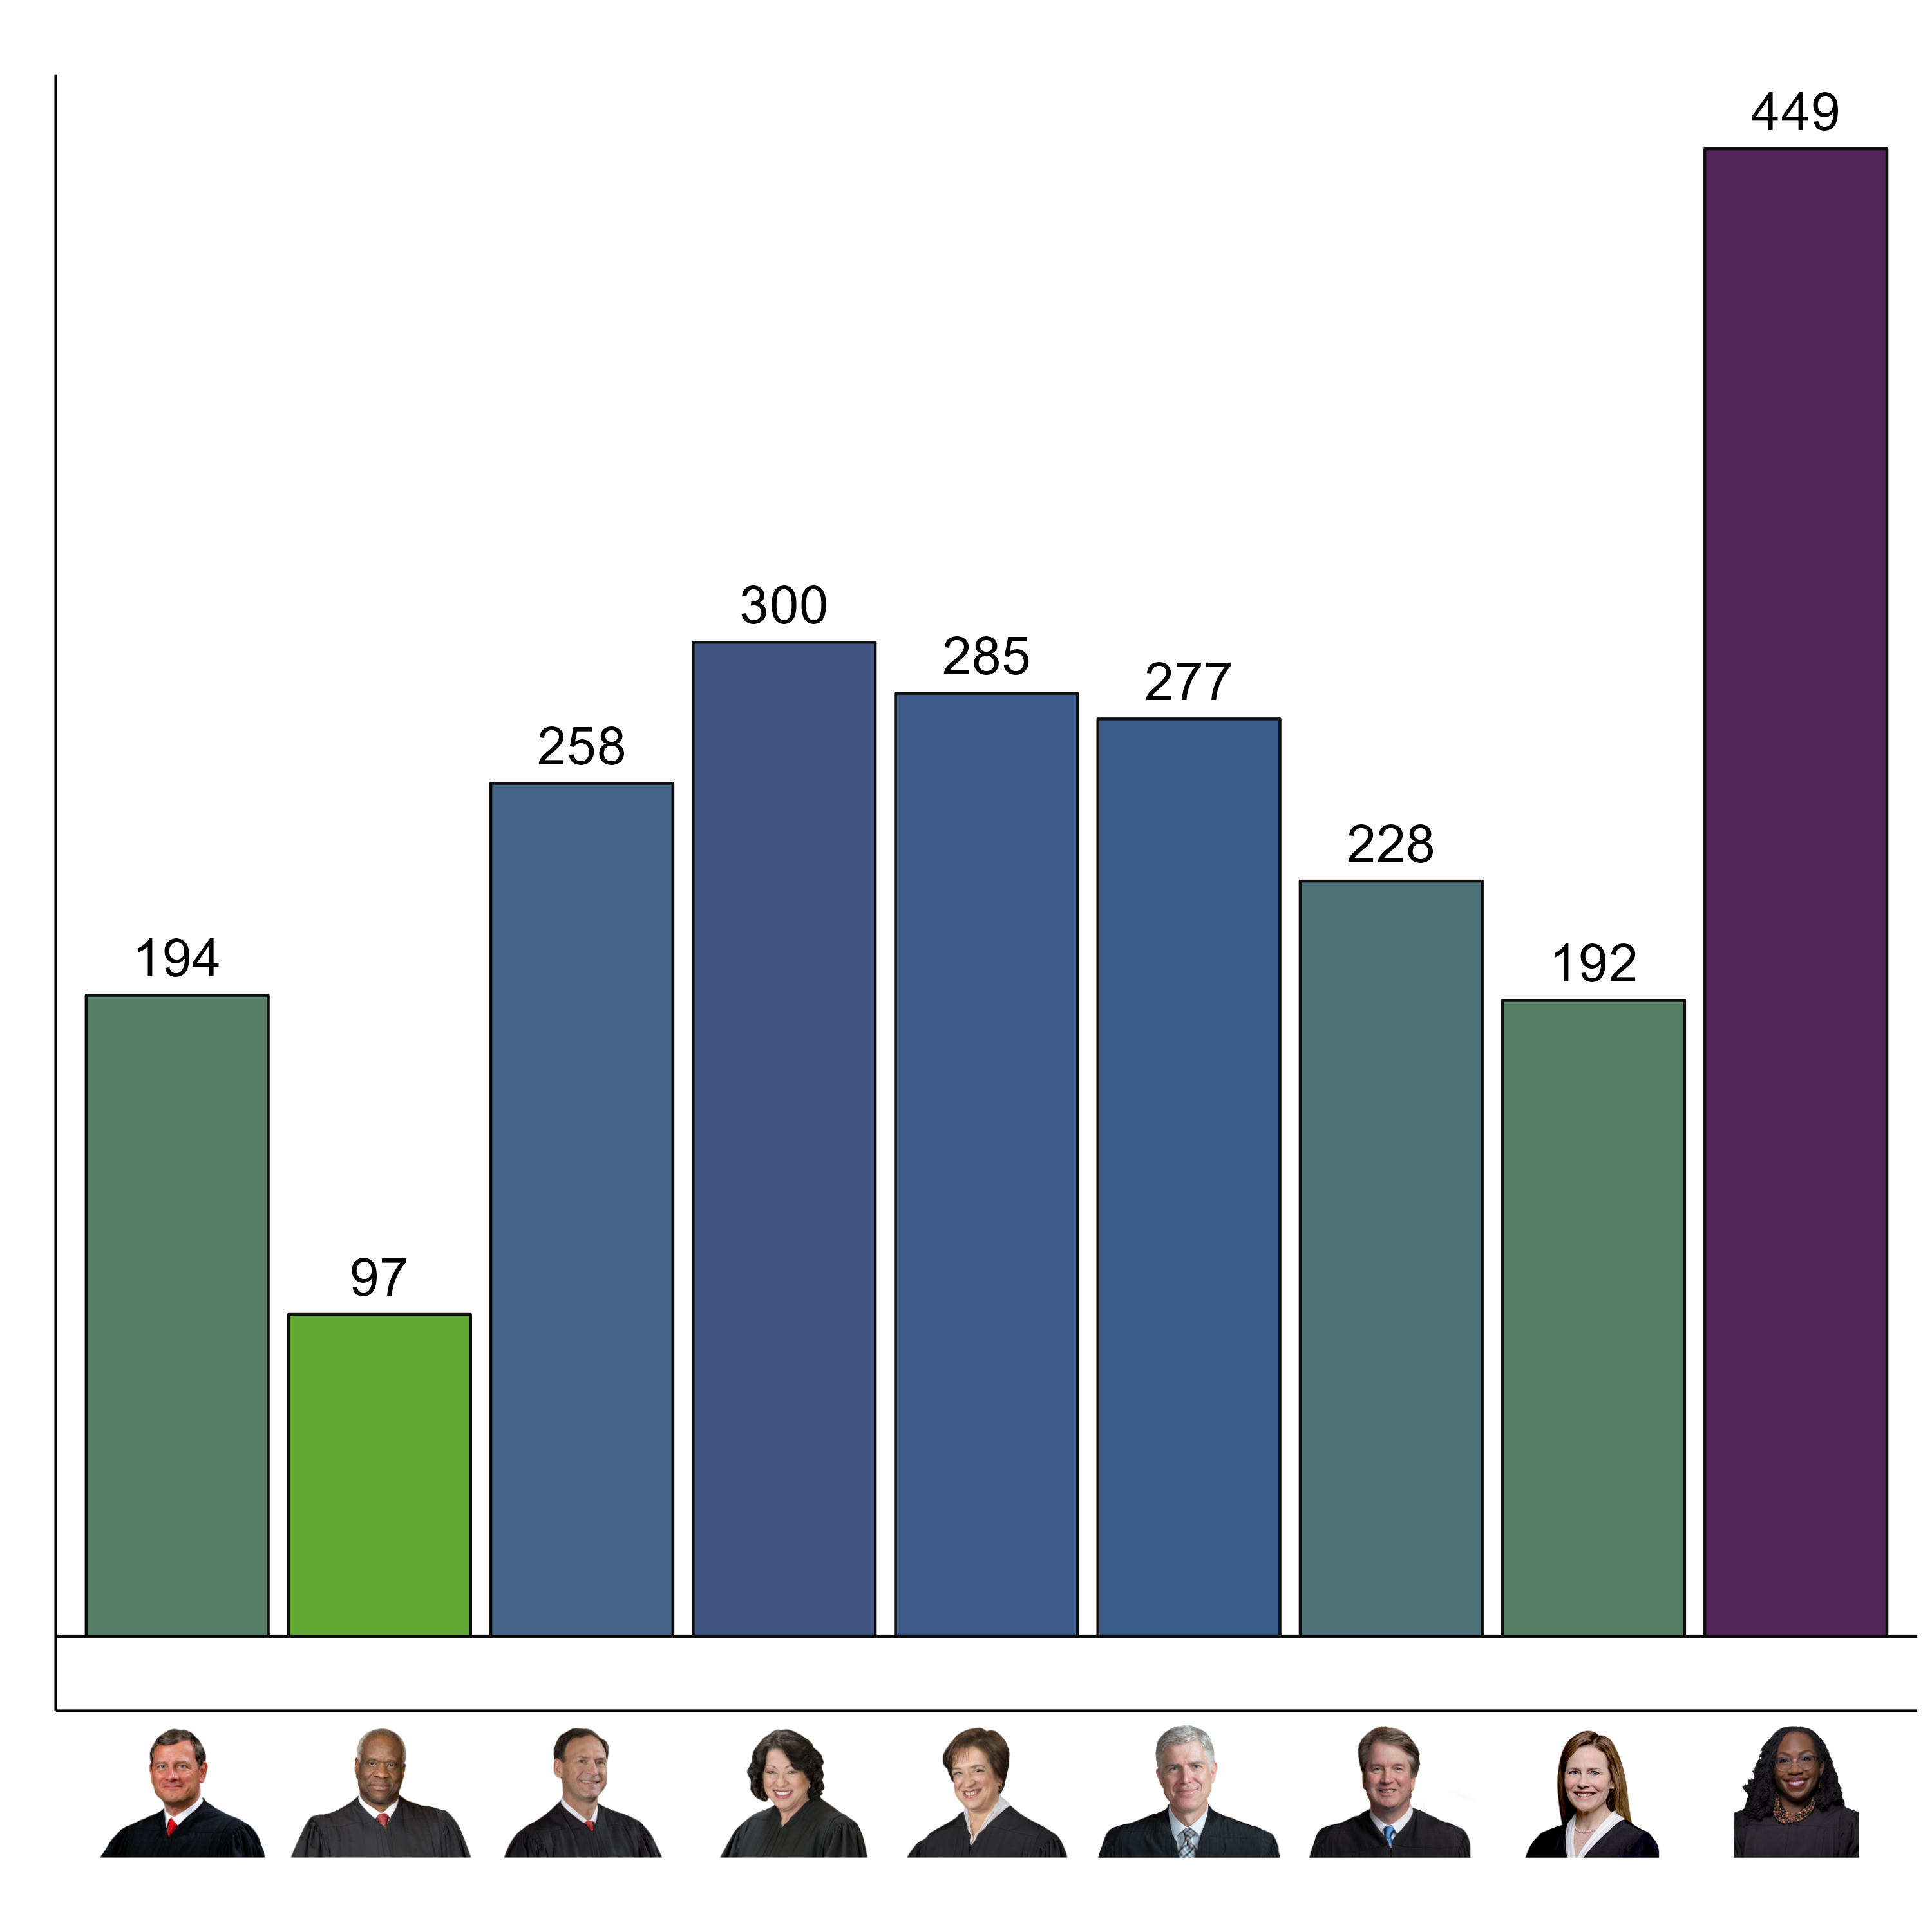
\includegraphics[width = 0.85\textwidth]{"Figures/statpack_figures/total_time_spoken_plot_OT23.png"} \\
\footnotesize{Data Source: Compiled from Oyez}
\end{figure}
\newpage


\begin{table}[H]
    \centering
    \renewcommand{\arraystretch}{1.5} % Add space between rows
    \caption{October Sitting (Time Spoken -- Minutes)}
    \vspace{2mm}
    \csvreader[
        tabular= {L{0.25\textwidth}cccccccccc}, % Left-align the first column, Center-align rows 2 to 10
        table head = {
            \toprule
            \multicolumn{1}{c}{} &
            \multirow{2}{*}{} &
            \multirow{2}{*}{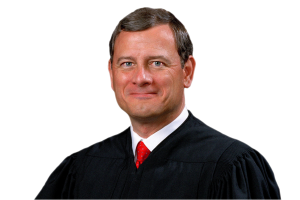
\includegraphics[width=1.5cm]{"Figures/justice_images/Roberts.png"}} &
            \multirow{2}{*}{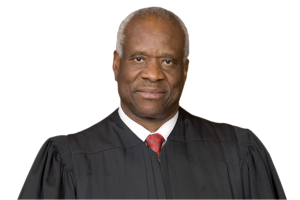
\includegraphics[width=1.5cm]{"Figures/justice_images/Thomas.png"}} &
            \multirow{2}{*}{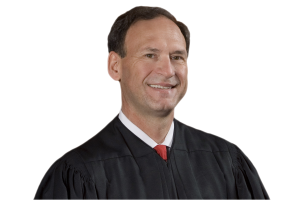
\includegraphics[width=1.5cm]{"Figures/justice_images/Alito.png"}} &
            \multirow{2}{*}{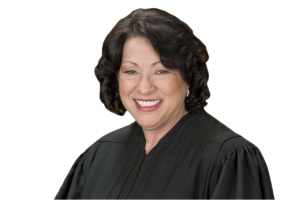
\includegraphics[width=1.5cm]{"Figures/justice_images/Sotomayor.png"}} &
            \multirow{2}{*}{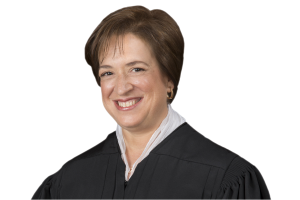
\includegraphics[width=1.5cm]{"Figures/justice_images/Kagan.png"}} &
            \multirow{2}{*}{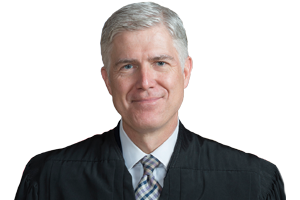
\includegraphics[width=1.5cm]{"Figures/justice_images/Gorsuch.png"}} &
            \multirow{2}{*}{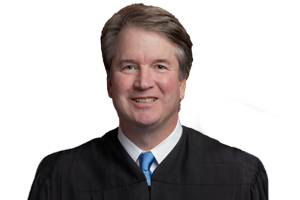
\includegraphics[width=1.5cm]{"Figures/justice_images/Kavanaugh.png"}} &
            \multirow{2}{*}{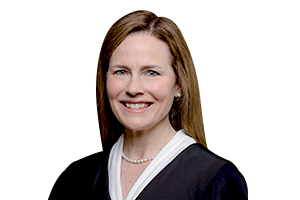
\includegraphics[width=1.5cm]{"Figures/justice_images/Barrett.png"}} &
            \multirow{2}{*}{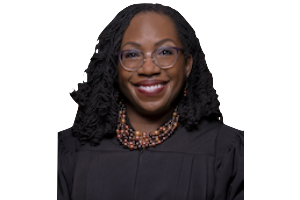
\includegraphics[width=1.5cm]{"Figures/justice_images/Jackson.png"}} \\
            \addlinespace
            \addlinespace
            & \footnotesize{Total} & \footnotesize{Roberts} & \footnotesize{Thomas} & \footnotesize{Alito} & \footnotesize{Sotomayor} & \footnotesize{Kagan} & \footnotesize{Gorsuch} & \footnotesize{Kavanaugh} & \footnotesize{Barrett} & \footnotesize{Jackson} \\
            \cmidrule{2-11}
        },
        table foot=\bottomrule \multicolumn{11}{l}{\footnotesize{\emph{Note}: \emph{Total} represents elapsed speaking time for entire argument (not including arguing attorneys) -- Does \emph{not} include empty (silent) space.}} \\ \multicolumn{11}{l}{\footnotesize{Data Source: Compiled from Oyez}} \\ \bottomrule % Specify the footer rule
    ]{"Tables/oral_argument_speaking/oral_argument_speaking_times_October.csv"}{}%
    {\footnotesize \csvcoli & \multirow{1}{*}{\centering\csvcolii} & \multirow{1}{*}{\centering\csvcoliii} & \multirow{1}{*}{\centering\csvcoliv} & \multirow{1}{*}{\centering\csvcolv} & \multirow{1}{*}{\centering\csvcolvi} & \multirow{1}{*}{\centering\csvcolvii} & \multirow{1}{*}{\centering\csvcolviii} & \multirow{1}{*}{\centering\csvcolix} & \multirow{1}{*}{\centering\csvcolx} & \multirow{1}{*}{\centering\csvcolxi}} % Specify all columns to include
    \label{tab:yourlabel}
\end{table}


\begin{table}[H]
    \centering
    \renewcommand{\arraystretch}{1.5} % Add space between rows
    \caption{November Sitting (Time Spoken -- Minutes)}
    \vspace{2mm}
    \csvreader[
        tabular= {L{0.25\textwidth}cccccccccc}, % Left-align the first column, Center-align rows 2 to 10
        table head = {
            \toprule
            \multicolumn{1}{c}{} &
            \multirow{2}{*}{} &
            \multirow{2}{*}{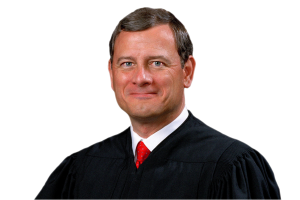
\includegraphics[width=1.5cm]{"Figures/justice_images/Roberts.png"}} &
            \multirow{2}{*}{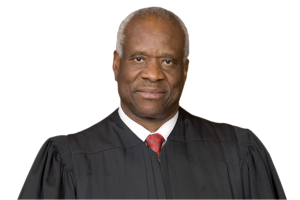
\includegraphics[width=1.5cm]{"Figures/justice_images/Thomas.png"}} &
            \multirow{2}{*}{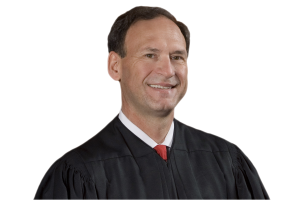
\includegraphics[width=1.5cm]{"Figures/justice_images/Alito.png"}} &
            \multirow{2}{*}{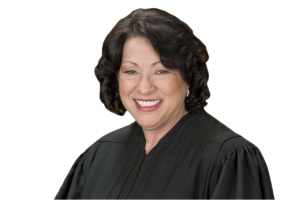
\includegraphics[width=1.5cm]{"Figures/justice_images/Sotomayor.png"}} &
            \multirow{2}{*}{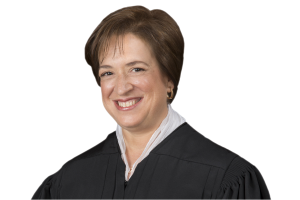
\includegraphics[width=1.5cm]{"Figures/justice_images/Kagan.png"}} &
            \multirow{2}{*}{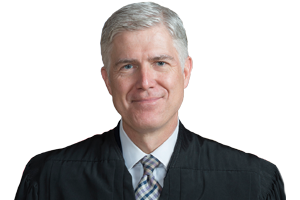
\includegraphics[width=1.5cm]{"Figures/justice_images/Gorsuch.png"}} &
            \multirow{2}{*}{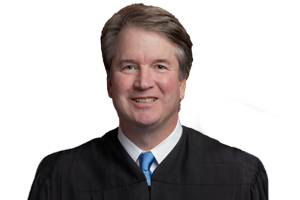
\includegraphics[width=1.5cm]{"Figures/justice_images/Kavanaugh.png"}} &
            \multirow{2}{*}{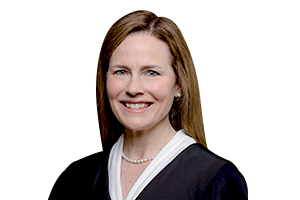
\includegraphics[width=1.5cm]{"Figures/justice_images/Barrett.png"}} &
            \multirow{2}{*}{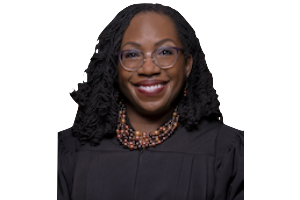
\includegraphics[width=1.5cm]{"Figures/justice_images/Jackson.png"}} \\
            \addlinespace
            \addlinespace
            & \footnotesize{Total} & \footnotesize{Roberts} & \footnotesize{Thomas} & \footnotesize{Alito} & \footnotesize{Sotomayor} & \footnotesize{Kagan} & \footnotesize{Gorsuch} & \footnotesize{Kavanaugh} & \footnotesize{Barrett} & \footnotesize{Jackson} \\
            \cmidrule{2-11}
        },
        table foot=\bottomrule \multicolumn{11}{l}{\footnotesize{\emph{Note}: \emph{Total} represents elapsed speaking time for entire argument (not including arguing attorneys) -- Does \emph{not} include empty (silent) space.}} \\ \multicolumn{11}{l}{\footnotesize{Data Source: Compiled from Oyez}} \\ \bottomrule % Specify the footer rule
    ]{"Tables/oral_argument_speaking/oral_argument_speaking_times_November.csv"}{}%
    {\footnotesize \csvcoli & \multirow{1}{*}{\centering\csvcolii} & \multirow{1}{*}{\centering\csvcoliii} & \multirow{1}{*}{\centering\csvcoliv} & \multirow{1}{*}{\centering\csvcolv} & \multirow{1}{*}{\centering\csvcolvi} & \multirow{1}{*}{\centering\csvcolvii} & \multirow{1}{*}{\centering\csvcolviii} & \multirow{1}{*}{\centering\csvcolix} & \multirow{1}{*}{\centering\csvcolx} & \multirow{1}{*}{\centering\csvcolxi}} % Specify all columns to include
    \label{tab:yourlabel}
\end{table}



\begin{table}[H]
    \centering
    \renewcommand{\arraystretch}{1.5} % Add space between rows
    \caption{December Sitting (Time Spoken -- Minutes)}
    \vspace{2mm}
    \csvreader[
        tabular= {L{0.25\textwidth}cccccccccc}, % Left-align the first column, Center-align rows 2 to 10
        table head = {
            \toprule
            \multicolumn{1}{c}{} &
            \multirow{2}{*}{} &
            \multirow{2}{*}{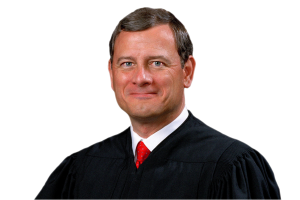
\includegraphics[width=1.5cm]{"Figures/justice_images/Roberts.png"}} &
            \multirow{2}{*}{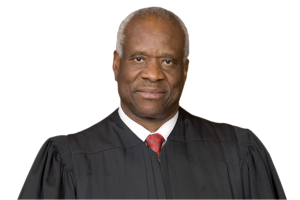
\includegraphics[width=1.5cm]{"Figures/justice_images/Thomas.png"}} &
            \multirow{2}{*}{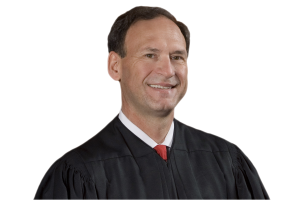
\includegraphics[width=1.5cm]{"Figures/justice_images/Alito.png"}} &
            \multirow{2}{*}{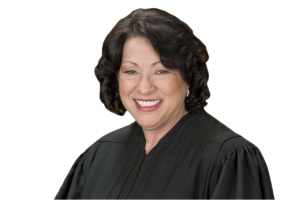
\includegraphics[width=1.5cm]{"Figures/justice_images/Sotomayor.png"}} &
            \multirow{2}{*}{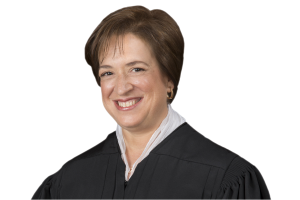
\includegraphics[width=1.5cm]{"Figures/justice_images/Kagan.png"}} &
            \multirow{2}{*}{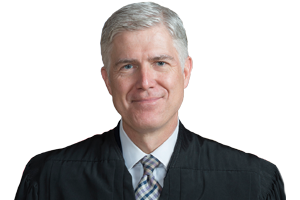
\includegraphics[width=1.5cm]{"Figures/justice_images/Gorsuch.png"}} &
            \multirow{2}{*}{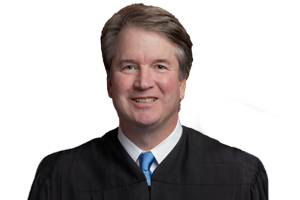
\includegraphics[width=1.5cm]{"Figures/justice_images/Kavanaugh.png"}} &
            \multirow{2}{*}{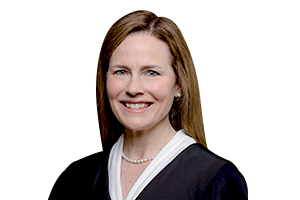
\includegraphics[width=1.5cm]{"Figures/justice_images/Barrett.png"}} &
            \multirow{2}{*}{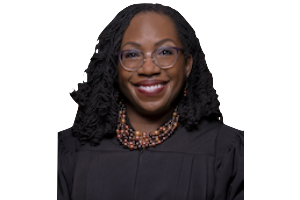
\includegraphics[width=1.5cm]{"Figures/justice_images/Jackson.png"}} \\
            \addlinespace
            \addlinespace
            & \footnotesize{Total} & \footnotesize{Roberts} & \footnotesize{Thomas} & \footnotesize{Alito} & \footnotesize{Sotomayor} & \footnotesize{Kagan} & \footnotesize{Gorsuch} & \footnotesize{Kavanaugh} & \footnotesize{Barrett} & \footnotesize{Jackson} \\
            \cmidrule{2-11}
        },
        table foot=\bottomrule \multicolumn{11}{l}{\footnotesize{\emph{Note}: \emph{Total} represents elapsed speaking time for entire argument (not including arguing attorneys) -- Does \emph{not} include empty (silent) space.}} \\ \multicolumn{11}{l}{\footnotesize{Data Source: Compiled from Oyez}} \\ \bottomrule % Specify the footer rule
    ]{"Tables/oral_argument_speaking/oral_argument_speaking_times_December.csv"}{}%
    {\footnotesize \csvcoli & \multirow{1}{*}{\centering\csvcolii} & \multirow{1}{*}{\centering\csvcoliii} & \multirow{1}{*}{\centering\csvcoliv} & \multirow{1}{*}{\centering\csvcolv} & \multirow{1}{*}{\centering\csvcolvi} & \multirow{1}{*}{\centering\csvcolvii} & \multirow{1}{*}{\centering\csvcolviii} & \multirow{1}{*}{\centering\csvcolix} & \multirow{1}{*}{\centering\csvcolx} & \multirow{1}{*}{\centering\csvcolxi}} % Specify all columns to include
    \label{tab:yourlabel}
\end{table}



\begin{table}[H]
    \centering
    \renewcommand{\arraystretch}{1.5} % Add space between rows
    \caption{January Sitting (Time Spoken -- Minutes)}
    \vspace{2mm}
    \csvreader[
        tabular= {L{0.25\textwidth}cccccccccc}, % Left-align the first column, Center-align rows 2 to 10
        table head = {
            \toprule
            \multicolumn{1}{c}{} &
            \multirow{2}{*}{} &
            \multirow{2}{*}{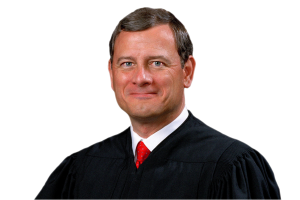
\includegraphics[width=1.5cm]{"Figures/justice_images/Roberts.png"}} &
            \multirow{2}{*}{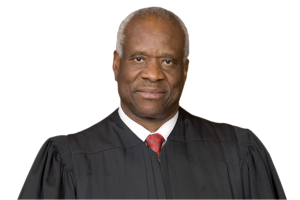
\includegraphics[width=1.5cm]{"Figures/justice_images/Thomas.png"}} &
            \multirow{2}{*}{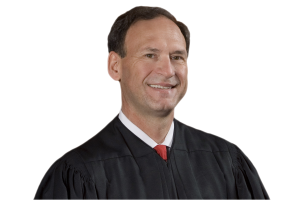
\includegraphics[width=1.5cm]{"Figures/justice_images/Alito.png"}} &
            \multirow{2}{*}{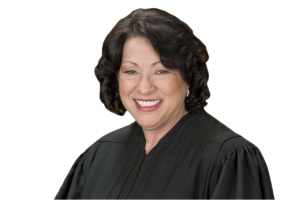
\includegraphics[width=1.5cm]{"Figures/justice_images/Sotomayor.png"}} &
            \multirow{2}{*}{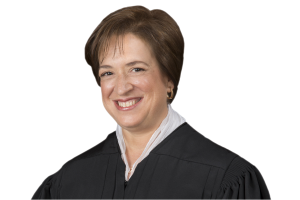
\includegraphics[width=1.5cm]{"Figures/justice_images/Kagan.png"}} &
            \multirow{2}{*}{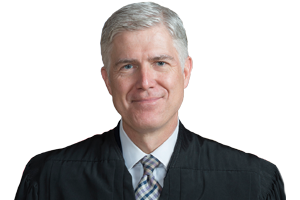
\includegraphics[width=1.5cm]{"Figures/justice_images/Gorsuch.png"}} &
            \multirow{2}{*}{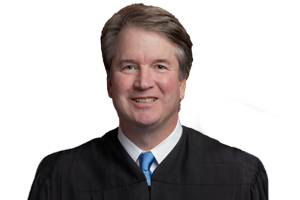
\includegraphics[width=1.5cm]{"Figures/justice_images/Kavanaugh.png"}} &
            \multirow{2}{*}{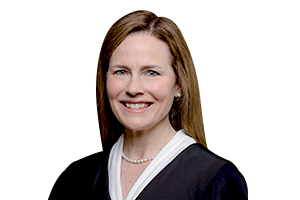
\includegraphics[width=1.5cm]{"Figures/justice_images/Barrett.png"}} &
            \multirow{2}{*}{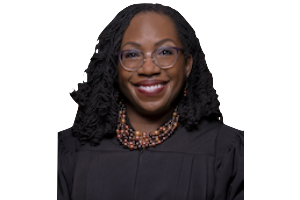
\includegraphics[width=1.5cm]{"Figures/justice_images/Jackson.png"}} \\
            \addlinespace
            \addlinespace
            & \footnotesize{Total} & \footnotesize{Roberts} & \footnotesize{Thomas} & \footnotesize{Alito} & \footnotesize{Sotomayor} & \footnotesize{Kagan} & \footnotesize{Gorsuch} & \footnotesize{Kavanaugh} & \footnotesize{Barrett} & \footnotesize{Jackson} \\
            \cmidrule{2-11}
        },
        table foot=\bottomrule \multicolumn{11}{l}{\footnotesize{\emph{Note}: \emph{Total} represents elapsed speaking time for entire argument (not including arguing attorneys) -- Does \emph{not} include empty (silent) space.}} \\ \multicolumn{11}{l}{\footnotesize{Data Source: Compiled from Oyez}} \\ \bottomrule % Specify the footer rule
    ]{"Tables/oral_argument_speaking/oral_argument_speaking_times_January.csv"}{}%
    {\footnotesize \csvcoli & \multirow{1}{*}{\centering\csvcolii} & \multirow{1}{*}{\centering\csvcoliii} & \multirow{1}{*}{\centering\csvcoliv} & \multirow{1}{*}{\centering\csvcolv} & \multirow{1}{*}{\centering\csvcolvi} & \multirow{1}{*}{\centering\csvcolvii} & \multirow{1}{*}{\centering\csvcolviii} & \multirow{1}{*}{\centering\csvcolix} & \multirow{1}{*}{\centering\csvcolx} & \multirow{1}{*}{\centering\csvcolxi}} % Specify all columns to include
    \label{tab:yourlabel}
\end{table}



\begin{table}[H]
    \centering
    \renewcommand{\arraystretch}{1.5} % Add space between rows
    \caption{February Sitting (Time Spoken -- Minutes)}
    \vspace{2mm}
    \csvreader[
        tabular= {L{0.25\textwidth}cccccccccc}, % Left-align the first column, Center-align rows 2 to 10
        table head = {
            \toprule
            \multicolumn{1}{c}{} &
            \multirow{2}{*}{} &
            \multirow{2}{*}{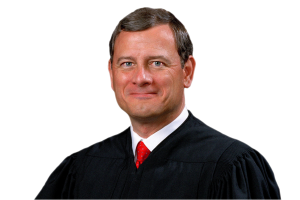
\includegraphics[width=1.5cm]{"Figures/justice_images/Roberts.png"}} &
            \multirow{2}{*}{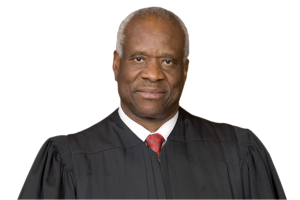
\includegraphics[width=1.5cm]{"Figures/justice_images/Thomas.png"}} &
            \multirow{2}{*}{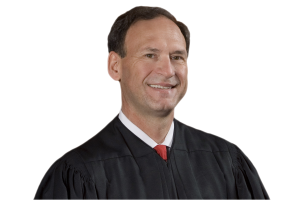
\includegraphics[width=1.5cm]{"Figures/justice_images/Alito.png"}} &
            \multirow{2}{*}{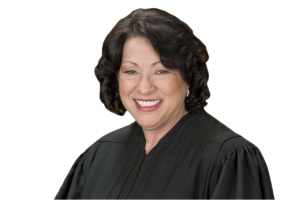
\includegraphics[width=1.5cm]{"Figures/justice_images/Sotomayor.png"}} &
            \multirow{2}{*}{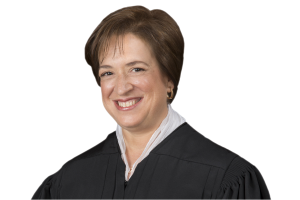
\includegraphics[width=1.5cm]{"Figures/justice_images/Kagan.png"}} &
            \multirow{2}{*}{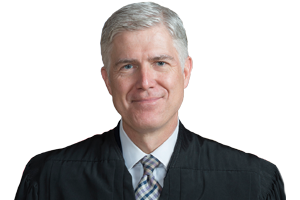
\includegraphics[width=1.5cm]{"Figures/justice_images/Gorsuch.png"}} &
            \multirow{2}{*}{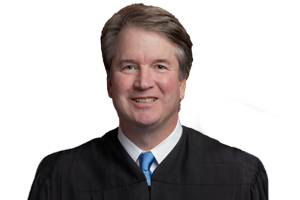
\includegraphics[width=1.5cm]{"Figures/justice_images/Kavanaugh.png"}} &
            \multirow{2}{*}{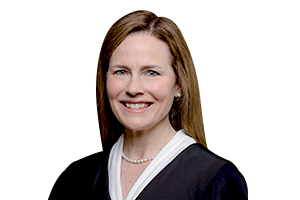
\includegraphics[width=1.5cm]{"Figures/justice_images/Barrett.png"}} &
            \multirow{2}{*}{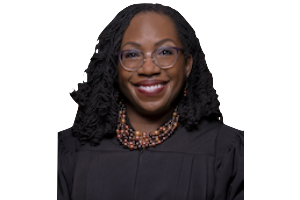
\includegraphics[width=1.5cm]{"Figures/justice_images/Jackson.png"}} \\
            \addlinespace
            \addlinespace
            & \footnotesize{Total} & \footnotesize{Roberts} & \footnotesize{Thomas} & \footnotesize{Alito} & \footnotesize{Sotomayor} & \footnotesize{Kagan} & \footnotesize{Gorsuch} & \footnotesize{Kavanaugh} & \footnotesize{Barrett} & \footnotesize{Jackson} \\
            \cmidrule{2-11}
        },
        table foot=\bottomrule \multicolumn{11}{l}{\footnotesize{\emph{Note}: \emph{Total} represents elapsed speaking time for entire argument (not including arguing attorneys) -- Does \emph{not} include empty (silent) space.}} \\ \multicolumn{11}{l}{\footnotesize{Data Source: Compiled from Oyez}} \\ \bottomrule % Specify the footer rule
    ]{"Tables/oral_argument_speaking/oral_argument_speaking_times_February.csv"}{}%
    {\footnotesize \csvcoli & \multirow{1}{*}{\centering\csvcolii} & \multirow{1}{*}{\centering\csvcoliii} & \multirow{1}{*}{\centering\csvcoliv} & \multirow{1}{*}{\centering\csvcolv} & \multirow{1}{*}{\centering\csvcolvi} & \multirow{1}{*}{\centering\csvcolvii} & \multirow{1}{*}{\centering\csvcolviii} & \multirow{1}{*}{\centering\csvcolix} & \multirow{1}{*}{\centering\csvcolx} & \multirow{1}{*}{\centering\csvcolxi}} % Specify all columns to include
    \label{tab:yourlabel}
\end{table}



\begin{table}[H]
    \centering
    \renewcommand{\arraystretch}{1.5} % Add space between rows
    \caption{March Sitting (Time Spoken -- Minutes)}
    \vspace{2mm}
    \csvreader[
        tabular= {L{0.25\textwidth}cccccccccc}, % Left-align the first column, Center-align rows 2 to 10
        table head = {
            \toprule
            \multicolumn{1}{c}{} &
            \multirow{2}{*}{} &
            \multirow{2}{*}{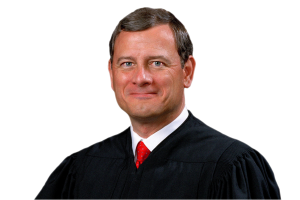
\includegraphics[width=1.5cm]{"Figures/justice_images/Roberts.png"}} &
            \multirow{2}{*}{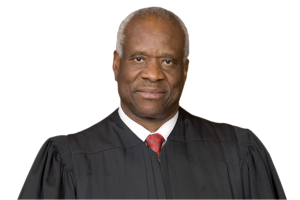
\includegraphics[width=1.5cm]{"Figures/justice_images/Thomas.png"}} &
            \multirow{2}{*}{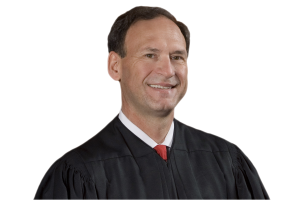
\includegraphics[width=1.5cm]{"Figures/justice_images/Alito.png"}} &
            \multirow{2}{*}{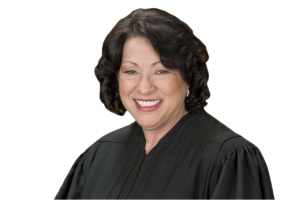
\includegraphics[width=1.5cm]{"Figures/justice_images/Sotomayor.png"}} &
            \multirow{2}{*}{\includegraphics[width=1.5cm]{"Figures/justice_images/Kagan.png"}} &
            \multirow{2}{*}{\includegraphics[width=1.5cm]{"Figures/justice_images/Gorsuch.png"}} &
            \multirow{2}{*}{\includegraphics[width=1.5cm]{"Figures/justice_images/Kavanaugh.png"}} &
            \multirow{2}{*}{\includegraphics[width=1.5cm]{"Figures/justice_images/Barrett.png"}} &
            \multirow{2}{*}{\includegraphics[width=1.5cm]{"Figures/justice_images/Jackson.png"}} \\
            \addlinespace
            \addlinespace
            & \footnotesize{Total} & \footnotesize{Roberts} & \footnotesize{Thomas} & \footnotesize{Alito} & \footnotesize{Sotomayor} & \footnotesize{Kagan} & \footnotesize{Gorsuch} & \footnotesize{Kavanaugh} & \footnotesize{Barrett} & \footnotesize{Jackson} \\
            \cmidrule{2-11}
        },
        table foot=\bottomrule \multicolumn{11}{l}{\footnotesize{\emph{Note}: \emph{Total} represents elapsed speaking time for entire argument (not including arguing attorneys) -- Does \emph{not} include empty (silent) space.}} \\ \multicolumn{11}{l}{\footnotesize{Data Source: Compiled from Oyez}} \\ \bottomrule % Specify the footer rule
    ]{"Tables/oral_argument_speaking/oral_argument_speaking_times_March.csv"}{}%
    {\footnotesize \csvcoli & \multirow{1}{*}{\centering\csvcolii} & \multirow{1}{*}{\centering\csvcoliii} & \multirow{1}{*}{\centering\csvcoliv} & \multirow{1}{*}{\centering\csvcolv} & \multirow{1}{*}{\centering\csvcolvi} & \multirow{1}{*}{\centering\csvcolvii} & \multirow{1}{*}{\centering\csvcolviii} & \multirow{1}{*}{\centering\csvcolix} & \multirow{1}{*}{\centering\csvcolx} & \multirow{1}{*}{\centering\csvcolxi}} % Specify all columns to include
    \label{tab:yourlabel}
\end{table}



\begin{table}[H]
    \centering
    \renewcommand{\arraystretch}{1.5} % Add space between rows
    \caption{April Sitting (Time Spoken -- Minutes)}
    \vspace{2mm}
    \csvreader[
        tabular= {L{0.25\textwidth}cccccccccc}, % Left-align the first column, Center-align rows 2 to 10
        table head = {
            \toprule
            \multicolumn{1}{c}{} &
            \multirow{2}{*}{} &
            \multirow{2}{*}{\includegraphics[width=1.5cm]{"Figures/justice_images/Roberts.png"}} &
            \multirow{2}{*}{\includegraphics[width=1.5cm]{"Figures/justice_images/Thomas.png"}} &
            \multirow{2}{*}{\includegraphics[width=1.5cm]{"Figures/justice_images/Alito.png"}} &
            \multirow{2}{*}{\includegraphics[width=1.5cm]{"Figures/justice_images/Sotomayor.png"}} &
            \multirow{2}{*}{\includegraphics[width=1.5cm]{"Figures/justice_images/Kagan.png"}} &
            \multirow{2}{*}{\includegraphics[width=1.5cm]{"Figures/justice_images/Gorsuch.png"}} &
            \multirow{2}{*}{\includegraphics[width=1.5cm]{"Figures/justice_images/Kavanaugh.png"}} &
            \multirow{2}{*}{\includegraphics[width=1.5cm]{"Figures/justice_images/Barrett.png"}} &
            \multirow{2}{*}{\includegraphics[width=1.5cm]{"Figures/justice_images/Jackson.png"}} \\
            \addlinespace
            \addlinespace
            & \footnotesize{Total} & \footnotesize{Roberts} & \footnotesize{Thomas} & \footnotesize{Alito} & \footnotesize{Sotomayor} & \footnotesize{Kagan} & \footnotesize{Gorsuch} & \footnotesize{Kavanaugh} & \footnotesize{Barrett} & \footnotesize{Jackson} \\
            \cmidrule{2-11}
        },
        table foot=\bottomrule \multicolumn{11}{l}{\footnotesize{\emph{Note}: \emph{Total} represents elapsed speaking time for entire argument (not including arguing attorneys) -- Does \emph{not} include empty (silent) space.}} \\ \multicolumn{11}{l}{\footnotesize{Data Source: Compiled from Oyez}} \\ \bottomrule % Specify the footer rule
    ]{"Tables/oral_argument_speaking/oral_argument_speaking_times_April.csv"}{}%
    {\footnotesize \csvcoli & \multirow{1}{*}{\centering\csvcolii} & \multirow{1}{*}{\centering\csvcoliii} & \multirow{1}{*}{\centering\csvcoliv} & \multirow{1}{*}{\centering\csvcolv} & \multirow{1}{*}{\centering\csvcolvi} & \multirow{1}{*}{\centering\csvcolvii} & \multirow{1}{*}{\centering\csvcolviii} & \multirow{1}{*}{\centering\csvcolix} & \multirow{1}{*}{\centering\csvcolx} & \multirow{1}{*}{\centering\csvcolxi}} % Specify all columns to include
    \label{tab:yourlabel}
\end{table}


\end{landscape}
